\documentclass[journal=jacsat,manuscript=article]{achemso}
\usepackage[latin1]{inputenc}
\usepackage{amsmath}
\usepackage{amsfonts}
\usepackage{amssymb}
\usepackage{graphicx}
\usepackage{numprint}
\usepackage{mathtools}
\usepackage{enumitem}
\usepackage{hyperref}
\usepackage[squaren,grey]{SIunits}
\usepackage{setspace}
\doublespacing

\author{Haina Wang}
\affiliation[Princeton University]{Department of Chemistry Torquato Lab, Princeton University, Princeton, NJ 08544, USA}
\email{hainaw@princeton.edu}

\title{Structure factors for some 1D--3D systems}
  
 
\begin{document}
	\maketitle
	\newpage
	\section{Introduction}
	The structure factor of a point process provides information of local density oscillations. Experimentally, it can be obtained through X-ray diffraction of materials. Mathematically, for a given point configuration with $N$ particles, the structure factor $S(\vec{k})$ of a wavevector $\vec{k}$ is defined by
	\begin{equation}
		S(\vec{k})=\frac{\vert\tilde{n}(\vec{k})\vert^2}{N}=\frac{\sum_{i=1}^{N}\sum_{j=1}^{N}e^{-i\vec{k}\cdot\left(\vec{r}_i-\vec{r}_j\right)}}{N}
	\end{equation}
	where $\vec{r}_i$ is the position of the $i$th particle in the system, and $\tilde{n}(\vec{k})=\sum_{i=1}^{N}e^{-i\vec{k}\cdot\vec{r_i}}$ is the Fourier transform of the local density function
	\begin{equation}
		n(\vec{r})=\sum_{i=1}^{N}\delta(\vec{r}-\vec{r}_i)
	\end{equation}
	
	The structure factor is related to the Fourier transform of the total correlation function $h(\vec{r})$ by
	\begin{equation}
		S(\vec{k})=1+\rho\tilde{h}(\vec{k})
	\end{equation}
	where $\rho=\frac{N}{V}$ is the number density. If the system is statistically homogeneous and statistically isotropic, $h(\vec{r})$ is a radial function. In this case, its Fourier transform is given by 
	\begin{equation}
		\tilde{h}(k)=(2\pi)^{\frac{d}{2}}\int_{0}^{\infty}r^{d-1}h(r)\frac{J_{d/2-1}(kr)}{(kr)^{d/2-1}}dr
	\end{equation}
	where $k=\vert\vec{k}\vert$ and $J_v(x)$ is the Bessel function of the first kind of order $v$.
	
	This report shows $S(\vec{k})$ of various ordered and disordered systems in 1--3 dimensions, including lattices, ideal gases, and equilibrium hard spheres.
	
	
	\newpage
	\section{1D lattice}
	The analytical structure factors were calculated by (1) for 1D systems with equidistant particles. The length of the cell is set to be $L=1$. The number of particles $N = 2,3,...,10$. The analytical results $S(k;N)$ are given explicitly below
	\begin{equation*}
		S(k;2)=\cos \left(\frac{k}{2}\right)+1
	\end{equation*}
	\begin{equation*}
		S(k;3)=\frac{1}{3} \left(2 \cos \left(\frac{k}{3}\right)+1\right)^2
	\end{equation*}
	\begin{equation*}
		S(k;4)=\left(\cos \left(\frac{k}{8}\right)+\cos \left(\frac{3 k}{8}\right)\right)^2
	\end{equation*}
	\begin{equation*}
		S(k;5)=\frac{1}{5} \left(2 \cos \left(\frac{k}{5}\right)+2 \cos \left(\frac{2 k}{5}\right)+1\right)^2
	\end{equation*}
	\begin{equation*}
		S(k;6)=\frac{2}{3} \left(\cos \left(\frac{k}{4}\right)+\cos \left(\frac{k}{12}\right)+\cos \left(\frac{5 k}{12}\right)\right)^2
	\end{equation*}
	\begin{equation*}
		S(k;7)=\frac{1}{7} \left(2 \cos \left(\frac{k}{7}\right)+2 \cos \left(\frac{2 k}{7}\right)+2 \cos \left(\frac{3 k}{7}\right)+1\right)^2
	\end{equation*}
	\begin{equation*}
		S(k;8)=\frac{1}{2} \left(\cos \left(\frac{k}{16}\right)+\cos \left(\frac{3 k}{16}\right)+\cos \left(\frac{5 k}{16}\right)+\cos \left(\frac{7 k}{16}\right)\right)^2
	\end{equation*}
	\begin{equation*}
		S(k;9)=\frac{1}{9} \left(2 \cos \left(\frac{k}{3}\right)+2 \cos \left(\frac{k}{9}\right)+2 \cos \left(\frac{2 k}{9}\right)+2 \cos \left(\frac{4 k}{9}\right)+1\right)^2
	\end{equation*}
	\begin{equation*}
		S(k;10)=\frac{2}{5} \left(\cos \left(\frac{k}{4}\right)+\cos \left(\frac{k}{20}\right)+\cos \left(\frac{3 k}{20}\right)+\cos \left(\frac{7 k}{20}\right)+\cos \left(\frac{9 k}{20}\right)\right)^2
	\end{equation*}
	
	In general, for 1D lattice with $N$ equidistant particles in a cell with length $L=1$, the expression for $S(k;N)$ is
	\begin{equation}
		S(k;N)=\frac{\sin ^2\left(\frac{k}{2}\right) \csc ^2\left(\frac{k}{2 N}\right)}{N}
	\end{equation}
	
	Fig. 1 plots the results. 
	
	\begin{figure}
		\includegraphics[width=1\linewidth]{sk1d}
		\caption{The analytical $S(k;N)$ versus $k$ of 1D lattice, where $N$ is the number of particles in the fundamental cell.}
		\label{fig:sk1d}
	\end{figure}

	The structure factor functions $S(k)$ are periodic. Gaussian-shaped peaks appear at $k$ values that are integral multiples of $\frac{2\pi}{L}$, where $L=\frac{1}{N}$ is the spacing between neighboring particles. The peak heights are $N$.
	 
	\section{2D lattices}
	The analytical structure factors for 2D square and triangular lattices with nearest neighbor distance 1 are shown in Fig. 2. We observe that peaks appear at the points of the "reciprocal lattice" of the corresponding lattices. For the square lattice, the reciprocal lattice is a square lattice rotated by $90^\circ$ with nearest neighbor distance $2\pi$. For the triangular lattice, the reciprocal lattice is another triangular lattice rotated by $30^\circ$ with nearest neighbor distance $\frac{4}{\sqrt{3}}\pi$.
	\begin{figure}
		\centering
		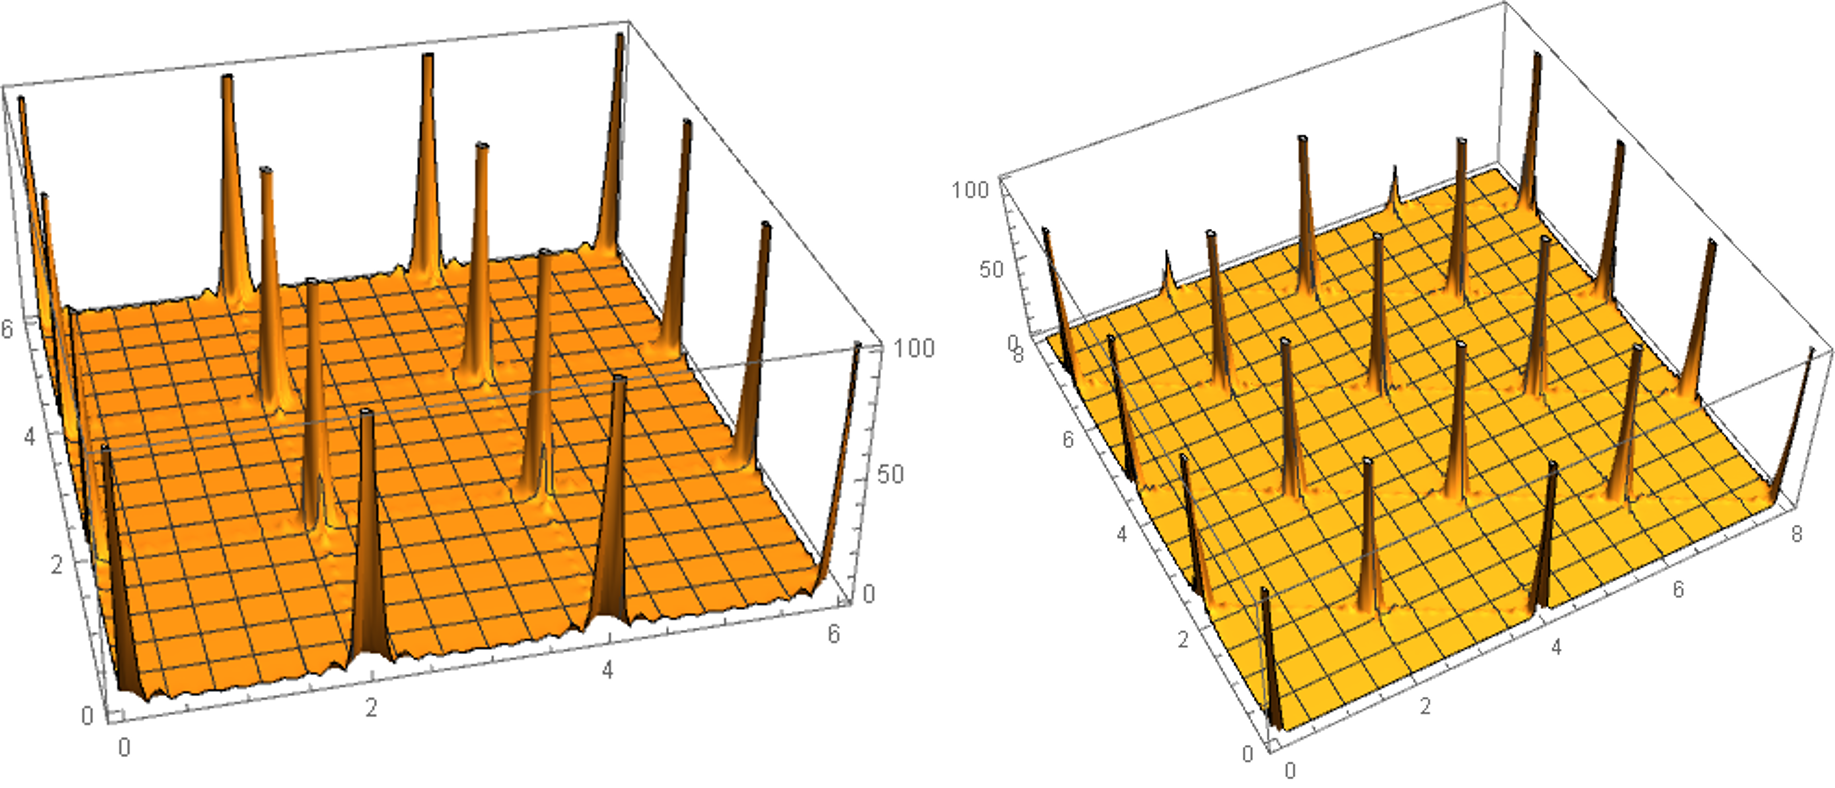
\includegraphics[width=1\linewidth]{lattice2D}
		\caption{The structure factors for 2D square and triangular lattices. The number of particles is $N=900$ for both cases. The generating vectors are (0,1) and (1,0) for the square lattice and $(1,0)$ and $\left(\frac{1}{2},\frac{\sqrt{3}}{2}\right)$ for the triangular lattice. Box dimensions are in multiples of $\pi$.}
		\label{fig:lattice2d}
	\end{figure}

	The angular averaged structure factor $S(k)$ for both lattices are given in Fig. 3. We note again the increase of peak heights with the number of particles in the fundamental cell.
	
	\begin{figure}
		\centering
		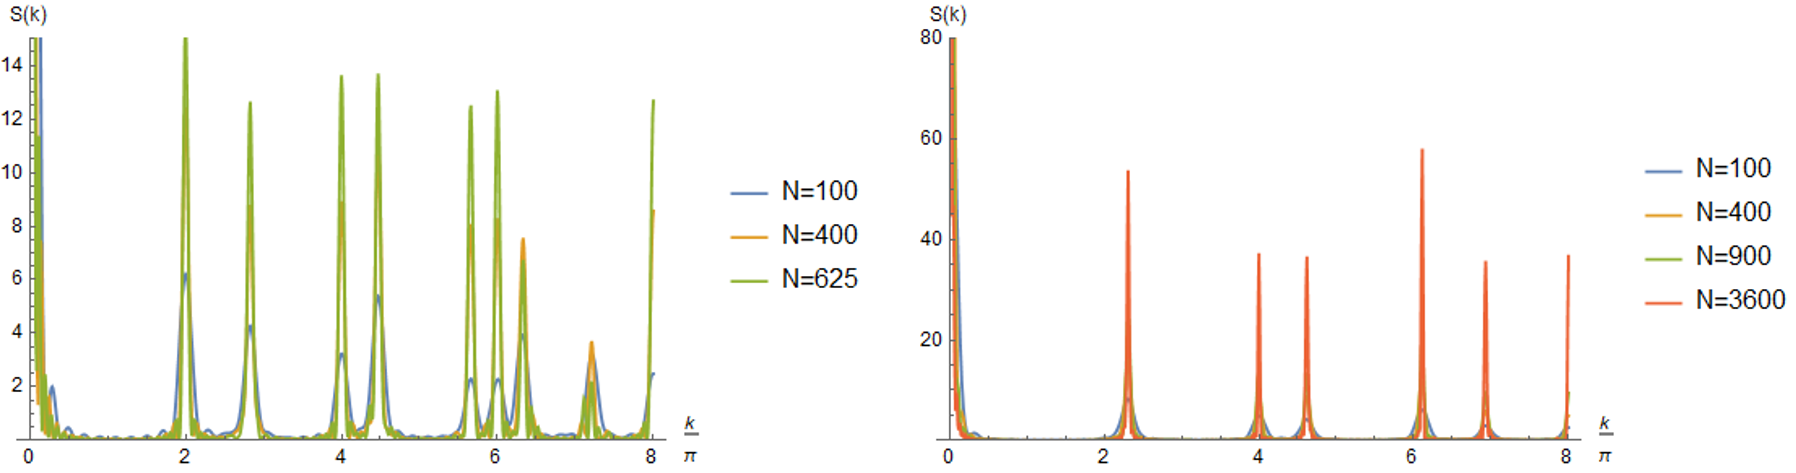
\includegraphics[width=1\linewidth]{lattice2DangAv}
		\caption{The angular averaged structure factor for the square and the triangular lattices. The generating vectors are (0,1) and (1,0) for the square lattice and $(1,0)$ and $\left(\frac{1}{2},\frac{\sqrt{3}}{2}\right)$ for the triangular lattice.}
		\label{fig:lattice2dangav}
	\end{figure}

	\newpage
	\section{Ideal gases}
	Fig. 4 shows the angular averaged structure factor for simulated ideal gas systems in 2D. Except from the forward scattering peak, the value of $S(k)$ is close to 1 almost everywhere regardless of the system size $N$. The result is very similar in 1D and 3D.
		
	\begin{figure}
		\centering
		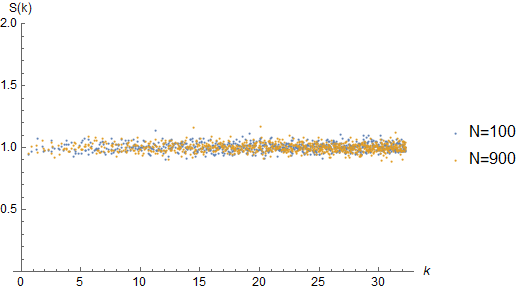
\includegraphics[width=1\linewidth]{ideal2D}
		\caption{The simulated structure factor for 2D ideal gases with various system size $N$. The fundamental cell side length is set to be 10.}
		\label{fig:ideal2d}
	\end{figure}
	
	\newpage
	\section{Equilibrium 3D hard spheres}
	The green curve in Fig. 5 shows the angular averaged $S(k)$ for equilibrium 3D hard spheres in the Percus--Yevick approximation with volume fraction $\phi=0.2$.
	
	Monte Carlo simulations were run with $N=1000$ in the fundamental cell. The particle diameters are set to be $D=1$. 50 equilibrium configurations were generated and $S(k)$ were computed in two different ways. 
	
	In one method, the total correlation function $h_2(r)=g_2(r)-1$ is first obtained by binning the pair distances. Then $S(k)$ is calculated by $S(k)=1+\rho \tilde{h}(k)$. The result for 50 configurations is averaged and plotted as the blue dashed curve in Fig. 5. This curve matches the PY approximation almost exactly where $k>2$. For $k<2$, $S(k)$ is underestimated.
	
	In the second method, $S(k)$ is directly computed from definition (1). The result for 50 configurations is averaged and plotted as red dots in Fig. 5. The data points also match the PY approximation very well for $k>1$.
	
	\begin{figure}
		\centering
		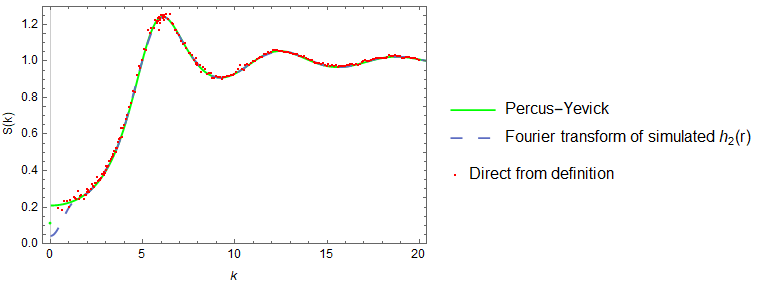
\includegraphics[width=1\linewidth]{C:/Users/Nora/Documents/G1.5/StrucFac/phi0_2}
		\caption{The angular averaged $S(k)$ for equilibrium 3D hard spheres with $\phi = 0.2$, $D=1$ in the Percus--Yevick approximation (green curve) , from the Fourier transform of simulated $h_2(r)$ (blue dashed curve), and from simulation and calculated directly from definition (1) (red dots). For simulations, system size $N=1000$.}
		\label{fig:theoreticalp0}
	\end{figure}
	
	\section{*Lennard--Jones systems: upcoming*}

	\newpage
	\section{Appendix}
	The codes and data are found in \url{https://github.com/Studio-Darboux-Carbonnier/StrucFac}.
\end{document}
